\documentclass[../main.tex]{subfiles}

\begin{document}

\chapter{正式踏入编程世界}

对于计算机小白而言,编程的世界可能会显得有些陌生和复杂。要想在这个世界中游刃有余,我们需要掌握的两个重要要素是\textbf{工具}和\textbf{环境}。

工具,指的是我们用来编写和运行程序的东西。包括语言、编辑器等。它们帮助我们更高效地达成我们的目标,例如调试程序、管理项目等。

环境,指的是我们编写和运行代码所依赖的操作系统、编程语言版本以及相关的库和框架。一个良好的编程环境可以大大提高我们的工作效率;同时,我们写出的代码,最终是也要运行在某个环境中的。编程语言本身就是为了让我们能够更方便地与计算机进行交流。

\section{编程语言初探}

\subsection{编程语言的发展简史}

编程语言的发展经历了几个重要阶段:

\begin{itemize}
  \item \textbf{机器语言}:最早的编程语言,直接与计算机硬件对应,使用二进制代码。最早的机器语言是通过拔插电缆实现的,是一个体力活,非常不便。后来改为采用打孔纸带的形式,但仍然非常繁琐和不直观。同时,对于不同的硬件架构,机器语言也不兼容,导致了可移植性差的问题。
  \item \textbf{汇编语言}:在机器语言基础上发展而来,引入了助记符,使得编程更加人性化。同时,汇编语言与特定的指令集相关联,这大大增强了其可移植性,但仍然需要对硬件有一定的了解。汇编语言虽然比机器语言更易读,但仍然需要手动管理内存和硬件资源。
  \item \textbf{高级语言}:高级语言的出现使得编程过程更像说话,而不是在机器上进行什么精确控制硬件的操作,显著增强了其可维护性和可读性;同时同一个高级语言在不同的硬件平台上只需要一个编译器或解释器,就可以运行,这也大大增强了其可移植性。高级语言可以分为两类:
        \begin{itemize}
          \item \textbf{编译型语言}:如C系语言,代码在运行前需要经过编译器转换为机器码,这样可以提高运行效率,但编译过程可能较慢。
          \item \textbf{解释型语言}:如Python,代码在运行时由解释器逐行解释执行,虽然运行速度可能较慢,但开发效率更高,调试更方便。
        \end{itemize}
\end{itemize}

现代的编程语言通常结合了编译型和解释型的优点,提供了更高的抽象层次和更丰富的功能库,使得编程变得更加高效和便捷。微软的.NET系就是一个典型的例子,它提供了一个统一的编程环境,支持多种语言,并且可以在不同的平台上运行。

\subsection{编程语言的特点和选择}

不同的编程语言往往有着自己的特点,选择合适的语言取决于项目需求和个人偏好。

一般情况下,涉及到底层硬件操作、性能要求高的项目,通常会选择编译型语言,如C/C++、Rust等。这些语言提供了对内存和硬件的直接控制,能够实现高效的性能优化;而对于快速开发、原型设计等任务,解释型语言如Python或JavaScript则更为合适。

除了这些通用性语言,还有一些语言能够对特定内容进行极好的支持,例如C\#用于游戏开发,LaTeX用于排版,SQL用于数据库查询,MatLab用于科学计算和数据分析,R用于统计分析等。这些语言通常在特定领域内有着广泛的应用。

不过归根结底,编程语言只是工具。初学者在学习编程的时候,更应该关注的是编程的思想和方法,而不是具体的编程语言。每一门语言都有自己的长处和缺点,在实际使用的时候应该具体情况具体应对。

\section{编程环境的搭建}

编程环境的搭建是编程的第一步。一个良好的编程环境可以大大提高我们的工作效率。

在搭建编程环境之前,我们应当先认识“环境变量”,它是操作系统中存储的变量,用于配置程序运行环境。环境变量可以影响程序的行为,例如指定编译器的路径、设置库文件的搜索路径等。

特别注意:\textbf{系统,尤其是Windows系统是一个很玄学的玩意},有时候需要重启计算机(或者终端)才能使环境变量生效,有时候则不需要。

\subsection{C系编译器及其环境配置}

对于C语言,有三个最常见的编译器:GCC、Clang和MSVC。它们各有特点,标准库略有不同,但都能满足大部分C语言开发的需求。我们一般建议在Linux上使用GCC,而在Mac上推荐使用Clang。MSVC工具链在Windows上非常流行,但是可移植性稍低,因此老派一点的程序员习惯不使用之,不过本质上没有什么区别。

Linux和Mac用户可以通过包管理器安装特定的编译器,在暑假课程的《包管理器》一节有讲授,这里不再赘述。

对于Windows用户,有两种方式获得这一编译器:如使用MSVC,则直接下载Visual Studio并安装C++开发模块即可,Visual Studio内置了MSVC工具链;如果使用GCC,则需要通过其他渠道。比起手动下载和配置GCC,我更推荐使用MSYS2或者Cygwin来安装GCC。它们提供了一个完整的Unix环境,免去了在Windows上配置编译器的麻烦。

你需要在\href{https://www.msys2.org/}{MSYS2官网}下载最新的安装包,并按照官网的说明进行安装。安装完成后,你可以通过MSYS2的包管理器pacman来安装GCC。

你可以在MSYS2终端中运行以下命令来安装GCC和GDB(建议使用UCRT64终端,不建议用其他的几个,剩下几个不知道什么时候就寄了):

\begin{verbatim}
pacman -S mingw-w64-x86_64-gcc
pacman -S mingw-w64-x86_64-gdb
\end{verbatim}

在MSYS2中安装完成后,用户如果想要在Windows终端中使用GCC,则需要设置环境变量,以便在命令行中直接使用编译器命令。

一般情况下,用户需要将MSYS2的bin目录添加到系统的PATH环境变量中。具体步骤如下:

\begin{itemize}
  \item 找到MSYS2的安装目录,通常是\texttt{C:\textbackslash msys64}。
  \item 将\texttt{C:\textbackslash msys64\textbackslash ucrt64\textbackslash bin}添加到系统的PATH环境变量中。
  \item 在PowerShell或者CMD中运行以下命令来验证是否配置成功:\texttt{gcc --version}。如果输出了GCC的版本信息,则说明配置成功。
  \item 如以上办法不起作用,可以尝试将\texttt{C:\textbackslash msys64\textbackslash usr\textbackslash bin}也添加到用户的PATH环境变量中。
\end{itemize}

\subsection{虚拟环境及其配置:以Python为例}

开发,尤其是生产类开发有一个重要的原则:不重复造轮子。以Python为例,作为一门流行的编程语言,它拥有丰富的第三方库和框架,可以帮助我们快速实现各种功能,并不需要从零开始开发。

因此,第三方库的安装和管理是开发中非常重要的一部分,而不同的开发往往需要不同的包,或者同一个包的不同版本。这些包有可能会产生冲突,如果用全局环境则会导致依赖混乱。这时,我们引入了虚拟环境,它是解决包冲突的有效手段。

虚拟环境可以理解为一个单独的盒子,包含了特定版本的编译器、解释器和所有依赖的包。用户可以在虚拟环境中自由安装和管理包,而不会影响全局的Python环境。一般有以下几种方法创建虚拟环境:
\begin{itemize}
  \item \textbf{venv}:Python内置的虚拟环境模块,适用于大多数场景。
  \item \textbf{virtualenv}:一个第三方库,提供了更多的功能和灵活性。
  \item \textbf{conda}:Anaconda发行版提供的虚拟环境管理工具,非常简洁高效,逐渐成为目前开发的主流选择。
  \item \textbf{docker}:容器化技术,可以将应用及其所有依赖打包在一个容器中,适用于生产环境,但是由于比较复杂、笨重、资源开销大,一般不推荐用于开发环境。
\end{itemize}

对于学生一般使用的是conda,或者其衍生高速版本mamba。我们的讲述也是以conda为主。

conda有两个发行版,一个是Anaconda,另一个是Miniconda。Anaconda包含了大量的预装包,适合初学者和数据科学家使用;而Miniconda则是一个轻量级的发行版,只包含conda和Python,适合需要自定义环境的用户。我们非常建议使用Miniconda,因为它更轻量,安装速度更快,并且可以根据需要安装所需的包。

特别注意的是,以上两个发行版在Linux和Winget上都难以利用包管理器进行安装。因此,我们一般都是直接从官网下载对应的安装包进行安装。安装完成后,用户需要设置环境变量,以便在命令行中直接使用conda命令。

接下来,因为一些原因,我们应当重启计算机(或者终端),以确保环境变量生效。

然后,我们需要进行终端初始化,例如在Windows上,我们可以使用以下命令:
\begin{verbatim}
    conda init powershell
\end{verbatim}

你应该将上述命令替换为你所使用的终端类型,例如在Linux上可以使用\texttt{bash}或\texttt{zsh}。然后你需要重启终端,以使初始化生效。

我们可以创建一个新的虚拟环境,例如:
\begin{verbatim}
    conda create -n myenv python=3.10
\end{verbatim}
这样就可以创建一个名为\texttt{myenv}的虚拟环境,并安装Python 3.10的尽可能新的版本。

下面我们需要激活虚拟环境:
\begin{verbatim}
    conda activate myenv
\end{verbatim}
这样就进入了虚拟环境,你可以在终端上看到提示符前面有\texttt{(myenv)},表示当前处于\texttt{myenv}虚拟环境中。如没有,可能是终端配置失败或者其他原因,安装OhMyPosh的部分主题也可能会导致这个问题(最大的可能是你的主题没有Python虚拟环境对应的section)。

现在在Python中我们一般流行使用\texttt{pip}来安装包,它从PyPI安装和管理第三方库。现在不流行直接使用conda管理包了。

我们可以使用以下命令安装一个包,例如安装\texttt{Numpy}库:
\begin{verbatim}
    pip install numpy
\end{verbatim}
这将会在当前虚拟环境中安装Numpy库,而不会影响全局的Python环境。

如果你需要安装多个包,可以将它们写在一个文件中,例如\texttt{requirements.txt},然后使用以下命令安装:
\begin{verbatim}
    pip install -r requirements.txt
\end{verbatim}
以上命令也常用于项目的依赖管理,可以方便地安装和更新项目所需的所有包;同时也可以通过修改\texttt{requirements.txt}文件来管理项目的依赖版本,适宜分发。

\section{选择合适的集成开发环境或者文本编辑器}

IDE(集成开发环境)或者文本编辑器是编程的核心工具之一,用于编写代码、调试和测试等功能。选择合适的IDE或编辑器可以提高编程效率和代码质量。

聪明的懒人宁可使用一天时间来把环境配好来节省以后的时间用来摸鱼,而不是天天花时间来鼓捣环境。

\subsection{选择编辑器}

最Geek的一批程序员最喜欢使用命令行编辑器,例如Vim、Emacs、NeoVim等。这些编辑器通常具有强大的功能和高度的可定制性,适合喜欢命令行操作和自定义配置的用户。但是这些编辑器的使用难度极高,学习曲线陡峭,对于初学者来说极不友好。StackOverflow上的一个非常著名的笑话是“Vim是一个非常强大的编辑器,但是你需要先学会如何退出它”。

题外话:退出Vim的命令是\texttt{:q},如果你在编辑器中输入了内容并且想要保存,可以使用\texttt{:wq}命令;如果你不想保存,可以使用\texttt{:q!}命令强制退出。

正课一般推荐的两个C++ IDE是Visual Studio和DevC++,Python IDE是PyCharm,它们各有各的优势,并且有一个最大的共同点:开箱即用。用户并不需要复杂的配置来进行编程。但是它们的缺点非常明显:

Visual Studio和PyCharm都非常臃肿,尤其是前者如果安装全家桶需要大量的磁盘空间和内存资源。同时,它们更注重于超大型项目的开发,这一“超大”往往动辄涉及数十万甚至上百万行代码,我们日常学习使用的代码量远远达不到这个级别,只能说是“杀鸡焉用牛刀”。VS的另一个缺点是它实际上专精于Windows平台和微软的.NET生态系统,虽然它也支持C++和Python等语言,但很笨。

DevC++是一个轻量级的C++ IDE,功能少得可怜,虽然比较适合初学者,但扩展性极差,无法满足更复杂的开发需求。它的界面和功能都比较简单,适合初学者入门,但对于需要更多功能和灵活性的用户来说,DevC++可能不够用。

因此,我并不推荐初学阶段就使用这些IDE。从长远来看,使用更加通用的编辑器会更有利于你在编程世界中游刃有余,例如Visual Studio Code(VSCode)。它是一款轻量级的编辑器,具有良好的扩展性和社区支持,可以满足不同用户的需求。VSCode支持多种编程语言,并且有丰富的插件生态系统,可以根据需要安装各种插件来增强功能。它的界面友好,易于上手,同时也提供了强大的调试和版本控制功能,非常适合初学者和中小型项目开发者使用。

除此之外,还有一些语言仅在特定的编辑器中有很好的支持,例如C\#之于Visual Studio,SQL之于DBeaver和DataGrip等。这些需要特定编辑器的语言通常在特定领域内有着广泛的应用。

\subsection{安装VS Code}

我们应该上官网下载安装包进行安装。我们需要安装的是System Installer版本,而不是User Installer版本。因为User Installer版本会将VS Code安装在用户目录下,而System Installer版本会将VS Code安装在系统目录下,这样可以方便地在所有用户之间共享VS Code,并且能够把它直接放在环境变量中。

安装完成后,我们需要设置环境变量,以便在命令行中直接使用code命令。不过如果你在安装时选择了“Add to PATH”选项,则不需要手动设置环境变量。

\subsection{配置VS Code}

VS Code是一个非常灵活的编辑器,可以通过安装插件来增强其功能。常用的插件包括:

\begin{itemize}
  \item \textbf{Python}:提供对Python的支持,包括语法高亮、代码补全、调试等功能。
  \item \textbf{C/C++}:提供对C/C++的支持,包括语法高亮、代码补全、调试等功能。
  \item \textbf{GitLens}:增强版的Git支持,可以更好地查看版本历史和代码变更。
\end{itemize}

此外,VS Code还支持多种主题和图标包,可以根据个人喜好进行定制。你可以在VS Code的插件市场中搜索并安装这些插件。

\subsubsection{在VS Code中配置GCC}

如果你使用的是GCC编译器,则需要在VS Code中配置GCC,以便能够编译和运行C/C++代码。可以通过以下步骤进行配置:

\begin{enumerate}
  \item 安装C/C++插件:在VS Code的插件市场中搜索并安装C/C++插件。建议直接安装微软提供的全家桶。
  \item 配置tasks.json文件:在VS Code中创建一个C++项目,然后随便输入一些什么代码。然后执行之,首次执行时VS Code会提示你创建一个\texttt{tasks.json}文件。选择“C/C++: g++.exe 生成活动文件”,这将会在项目根目录下创建一个\texttt{.vscode/tasks.json}文件。(如你使用的是MSVC,则选择“C/C++: cl.exe 生成活动文件”。)
  \item 配置launch.json文件:在VS Code中按下\texttt{F5},选择“C++ (GDB/LLDB)”,然后选择“g++.exe build and debug active file”。这将会在项目根目录下创建一个\texttt{.vscode/launch.json}文件。(如果没有后一步,可以忽略之。)
\end{enumerate}

如果你并不信任微软提供的配置文件,可以手动创建\texttt{tasks.json}和\texttt{launch.json}文件。这两个文件都应该放在项目根目录下的\texttt{.vscode}文件夹中。

以下是一个简单的\texttt{tasks.json}文件示例:

\begin{verbatim}
{
  "version": "2.0.0",
  "tasks": [
    {
      "label": "C/C++: g++.exe 生成活动文件",
      "type": "shell",
      "command": "g++",
      "args": [
        "-g",
        "${file}",
        "-o",
        "${fileDirname}\\${fileBasenameNoExtension}.exe"
      ],
      "group": {
        "kind": "build",
        "isDefault": true
      },
      "problemMatcher": ["$gcc"],
      "detail": "生成活动文件"
    }
  ]
}
\end{verbatim}

以下是一个简单的\texttt{launch.json}文件示例:

\begin{verbatim}
{
  "version": "0.2.0",
  "configurations": [
      {
          "name": "C++ Launch",
          "type": "cppdbg",
          "request": "launch",
          "program": "${fileDirname}\\${fileBasenameNoExtension}.exe",
          "args": [],
          "stopAtEntry": false,
          "cwd": "${workspaceFolder}",
          "environment": [],
          "externalConsole": false,
          "MIMode": "gdb",
          "setupCommands": [
              {
                  "description": "Enable pretty-printing for gdb",
                  "text": "-enable-pretty-printing",
                  "ignoreFailures": true
              }
          ],
          "preLaunchTask": "C/C++: g++.exe 生成活动文件",
          "miDebuggerPath": "C:\\msys64\\ucrt64\\bin\\gdb.exe"
      }
  ]
}
\end{verbatim}

\subsubsection{在VS Code中配置Python}

在VS Code中配置Python非常简单。只需要安装微软提供的三个Python插件,然后在VS Code中打开一个Python文件。

你会在右下角看到一个黄色按钮“选择Python解释器”,点击它可以选择你想要使用的Python解释器。一般情况下,你可以选择“Python 3.x (conda)”或者“Python 3.x (venv)”等选项,这样VS Code就会自动识别你当前的虚拟环境。

当然,我们非常建议同学们趁早熟悉纯命令行运行Python的方式,例如\texttt{python main.py},这样可以更好地理解Python的运行机制,同时也更便于调试(?)。

\subsubsection{在VS Code中配置Git}

在VS Code中配置Git同样非常简单。只需要安装Git,并确保Git的可执行文件在系统的PATH环境变量中。然后在VS Code中打开一个Git仓库,VS Code会自动识别并启用Git功能。

\section{美化你的终端}

在Windows上,默认的终端是cmd或者PowerShell,它们的界面比较简陋,不能显示很多信息。为了让终端更美观、更实用,我们可以使用一些终端美化工具,这里我推荐使用\textbf{Oh My Posh}。

\subsection{安装Oh My Posh}

我们建议使用winget来安装Oh My Posh。你可以在PowerShell中运行以下命令来安装:

\begin{verbatim}
  winget install JanDeDobbeleer.OhMyPosh
\end{verbatim}

安装完成后,你需要在PowerShell中运行以下命令来初始化Oh My Posh:
\begin{verbatim}
  oh-my-posh init pwsh | out-string | Invoke-Expression
\end{verbatim}

一般的计算机会阻止用户执行类似\texttt{Invoke-Expression}的命令,因此你需要在PowerShell中运行以下命令来允许执行:
\begin{verbatim}
  Set-ExecutionPolicy -ExecutionPolicy RemoteSigned -Scope CurrentUser
\end{verbatim}
上述命令的意思是允许当前用户执行远程签名的脚本。

如果你使用的是其他终端,例如cmd或者Git Bash,你可以在Oh My Posh的\href{https://ohmyposh.dev/docs/installation}{安装文档}中找到相应的安装方法。

\subsection{配置Oh My Posh}

首先,你应该安装OMP推荐使用的字体,例如Nerd Font。这是因为Oh My Posh使用了一些特殊的图标,如果没有合适的字体,可能会导致图标无法正常显示。

你可以在\href{https://www.nerdfonts.com/}{Nerd Fonts官网}下载最新的字体包。安装完成后,你需要在终端中设置字体为Nerd Font,以便能够正确显示Oh My Posh的图标。另一个办法是利用OhMyPosh安装这个字体:
\begin{verbatim}
  oh-my-posh font install meslo
\end{verbatim}

安装完成后,你需要在终端中设置字体为Nerd Font。以PowerShell为例,你可以右键点击窗口标题栏,选择“属性”,然后在“字体”选项卡中选择Nerd Font即可。

接下来,你可以在PowerShell中运行以下命令来设置Oh My Posh的主题:
\begin{verbatim}
  Set-PoshPrompt -Theme <theme-name>
\end{verbatim}

更多的主题可以在Oh My Posh的\href{https://ohmyposh.dev/docs/themes}{主题文档}中找到。你可以根据自己的喜好选择一个主题。 

\subsection{在VS Code中配置终端}

VS Code内置了终端功能,可以方便地在编辑器中运行命令。终端默认使用系统的命令行工具,例如在Windows上是cmd,在Linux上是bash。

你可以通过快捷键\texttt{Ctrl + `}(反引号)打开终端,也可以通过菜单\texttt{视图 > 终端}来打开。终端打开后,你可以在其中输入命令,和在普通命令行中一样。

如果你希望在VS Code中使用Oh My Posh,可以在VS Code的设置中将终端的默认shell设置为PowerShell。具体步骤如下:

\begin{enumerate}
  \item 打开VS Code的设置(可以通过快捷键\texttt{Ctrl + ,}打开)。
  \item 在搜索框中输入\texttt{terminal.integrated.shell.windows}。
  \item 将其值设置为\texttt{powershell}。
\end{enumerate}

如果你使用的是其他终端,例如Git Bash或者WSL,你可以将其值设置为相应的终端路径。

然后,你应该把Oh My Posh的初始化命令添加到PowerShell的配置文件中,以便每次打开PowerShell时都能自动加载Oh My Posh。你可以在PowerShell中运行以下命令来编辑配置文件:
\begin{verbatim}
  code $PROFILE
\end{verbatim}
以上代码会使用code命令打开PowerShell的配置文件。然后在文件末尾添加一些内容即可,具体内容详见\href{https://ohmyposh.dev/docs/installation/windows}{Oh My Posh的安装文档}。

下一步则是把Code的终端字体设置为Nerd Font。你可以在VS Code的设置中搜索\texttt{terminal.integrated.fontFamily},然后将其值设置为你安装的Nerd Font的名称,例如\texttt{MesloLGS Nerd Font}。


\section{编写程序的基本素养}

做了这么多操作,我们终于可以编写第一个能跑的程序了。我们将使用C++和Python两个语言来演示怎么书写第一个程序,同时告诉大家编程新手应有的素养。

\subsection{编写你的第一个程序}

由于众所周知的原因,我们的第一个程序通常是“Hello, World!”程序。它的作用是让我们熟悉编程语言的基本语法和编译运行流程,同时也是一个传统。而第二个程序一般往往是写一个加法,让我们熟悉输入输出的基本操作。

\subsubsection{C++}

对于C++,我们可以使用以下代码来编写第一个程序:

\begin{verbatim}
#include <iostream>
int main() {
    std::cout << "Hello, World!" << std::endl;
    return 0;
}
\end{verbatim}

然后如果配置得当,我们就可以通过按下F5键来编译并运行这个程序了。VS Code会自动调用编译器进行编译,并在终端中显示输出结果。如果一切顺利,你应该会看到“Hello, World!”的输出。

在一些极端情况下(例如无GUI环境),你可能需要手动编译和运行程序。可以使用以下命令来编译和运行程序:

\begin{verbatim}
g++ -o hello hello.cpp
./hello
\end{verbatim}

请使用类似的方式\textbf{手敲}、编译、运行以下代码:

\begin{verbatim}
#include <iostream>
int main() {
    int a, b;
    std::cout << "Enter the first integer: ";
    std::cin >> a;
    std::cout << "Enter the second integer: ";
    std::cin >> b;
    std::cout << "Their sum is: " << a + b << std::endl;
    return 0;
}
\end{verbatim}

\subsubsection{Python}

对于Python,我们同样可以使用以下代码来编写第一个程序:

\begin{verbatim}
print("Hello, World!")
\end{verbatim}

同样,如果配置得当,我们就可以通过按下F5键来运行这个程序了。VS Code会自动调用Python解释器进行运行,并在终端中显示输出结果。同样的,如果希望使用命令行来运行程序,可以使用以下命令:

\begin{verbatim}
python hello.py
\end{verbatim}

请使用类似的方式\textbf{手敲}、编译、运行以下代码:

\begin{verbatim}
a = int(input("Enter the first integer: "))
b = int(input("Enter the second integer: "))
print("Their sum is:", a + b)
\end{verbatim}

\subsubsection{这两个语言有什么区别?}

可以看到,使用命令行来执行程序的方式有所不同:C++需要两步,但是Python只需要一步。这是因为C++是编译型语言,需要先将源代码编译成可执行文件,然后再运行;而Python是解释型语言,直接运行源代码即可。前者的好处是,一份需要被反复运行的代码只需要编译一次,之后可以反复运行。而后者的好处是,代码修改后可以立即运行,但是需要反复解释执行,运行速度(相对的)非常缓慢。

另一个区别是,C++中,我们可以看到定义a和b之前需要先声明它们的类型,而Python中则不需要。这说明,C++是强类型语言,变量的类型在编译时就确定了;而Python是动态类型语言,变量的类型在运行时才确定。

而这也导致了一个问题:编译器可以识别全部的语法错误和部分的语义错误,因此一份能够编译通过的C++代码,通常代码本身是正确的,但是算法可能因为极端数据出现错误,例如除零等;而Python则无法检查语法错误和语义错误,解释器只会在按顺序运行代码,直到在出现问题的的地方停止。Python 自身的动态类型系统与缺少编译器带来的静态查错系统,使得实际写出来的 Python 代码中经常包含大量的错误。

\subsection{学会阅读错误信息}

从上文中我们知道,代码中出现错误是不可避免的一件事情。而很多情况下,我们在只有在代码跑起来的时候才能发现错误。此时,编译器或解释器会给出错误信息,帮助我们定位问题所在。

例如,以下是C++初学者常见的错误:

\begin{verbatim}
  #include<iostream>
  using namespace std;
  int mian()
  {
      cout<<"Hello World!"<<endl;
      return 0;
  }
\end{verbatim}

而它的错误信息是在编译时报出:

\begin{verbatim}
> g++ example.cpp -o example.exe

ld.exe: *.a(lib64_libmingw32_a-crtexewin.o): in function `main':
C:/.../crtexewin.c:70: undefined reference to `WinMain'
collect2.exe: error: ld returned 1 exit status
\end{verbatim}

虽然信息略显抽象,但我们还是可以看到很多有用的信息。 ld 是 C++ 中的链接器,再往上看可以发现对 WinMain 的引用是未定义的。这提示我们去看 main 函数,从而发现这里将\texttt{main}函数写成了\texttt{mian},因此链接器无法找到 main 函数,从而引发错误。

而Python给出的错误信息则更为直观,例如以下代码:

\begin{verbatim}
def calc(numbers):
  total = sum(numbers)
  count = len(numbers)
  return total / count

numbers = [10, 20, 30, 40, 50]
print("Average:", calc(numbers))

numbers.append("60")
print("Updated Average:", calc(numbers))
\end{verbatim}

其报错是:
\begin{verbatim}
Average: 30.0
Traceback (most recent call last):
  File "example.py", line 10, in <module>
    print("Updated Average:", calc(numbers))
  File "example.py", line 2, in calc
    total = sum(numbers)
TypeError: unsupported operand type(s) for +: 'int' and 'str'
\end{verbatim}

可以看到,解释器对第10行和第2行进行了报错。第10行的报错是因为在调用\texttt{calc}函数时,传入的\texttt{numbers}列表中包含了一个字符串“60”,而\texttt{calc}函数期望的是一个数字列表,因此在计算平均值时出现了类型错误(TypeError)。而第2行的报错则是因为在计算总和时,无法将整数和字符串相加。于是我们发现了问题所在:在第9行,我们向\texttt{numbers}列表中添加了一个字符串“60”,而不是一个数字。我们可以通过将其改为\texttt{numbers.append(60)}来解决这个问题。

顺便一提,这段代码在C++这种强类型语言中是无法通过编译的(\texttt{List<int>}类型不能进行append(string)),但 Python 的解释器还是运行代码直到遇到了具体的问题,在输出信息中可以看到第一个 \texttt{print()} 语句仍然被正常地执行。

\subsection{学会调试}

调试(技术人一般直接说debug)是我们发现和修复代码中隐藏起来的错误的最有力工具。调试可以帮助我们理解代码的执行流程,从而\textbf{定位}问题所在。

调试有两种手段:静态调试和动态调试。前者一般是通过静态分析工具(例如反汇编器)来分析代码的结构和逻辑,寻找潜在的问题;后者则是通过运行代码并观察其行为来发现问题。静态调试通常用于编译型语言且难度极高,我们不会涉及;而动态调试则适用于所有语言,接下来的内容我们将主要介绍动态调试。

C系有着自己的调试器:GDB(GNU Debugger),它是一个强大的调试工具,可以在命令行中使用。GDB可以让我们逐行执行代码,查看变量的值,设置断点等。VS Code也集成了GDB,可以通过图形界面进行调试。Python也有类似的调试器:PDB(Python Debugger),它同样可以在命令行中使用,也可以通过VS Code进行调试。

纯命令行调试的方式极为困难(尤其是GDB,需要背诵大量的命令),我们在这里不做介绍。然而,VS Code提供了一个非常友好的调试界面,可以通过图形化的方式进行调试。我们可以在代码中设置断点,逐行执行代码,查看变量的值等。这样可以大大提高调试效率。(当然这需要你安装GDB。)

安装GDB的方法也很简单,在Linux和Mac上可以通过包管理器安装,在Windows上可以通过MSYS2或Cygwin安装。安装完成后,我们需要在VS Code中配置GDB,以便能够使用图形化的方式进行调试。

一个较为简单的

我们调试主要有以下几个手段:打日志、打断点、写测试代码。

\subsubsection{打日志}

打日志是指在代码中添加打印语句,以便在运行时输出某些特定变量的值,进而确定程序的执行流程。这样可以帮助我们理解代码的执行过程,定位问题所在。

新人常常不喜欢这种手段,因为它需要在代码中添加额外的打印语句,很丑陋、不优雅,且会影响代码的可读性和维护性。但是打日志是一个非常有效的调试手段,尤其是在工程量巨大、无法或者很难打断点的情况下。

例如我在调试某数万行的大型项目时,出现assert错误。于是本人在代码中添加了以下打印语句:

\begin{figure}[htbp]
\centering
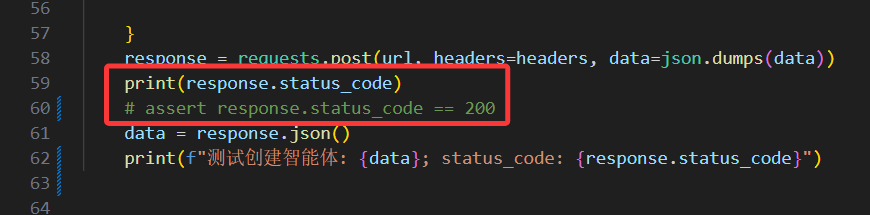
\includegraphics[width=0.8\textwidth]{images/printlog.png}
\caption{打日志的例子}
\end{figure}

这样我就知道了程序在执行到这里的时候,返回的不是预期的200,而是404。于是这让我顺藤摸瓜,排查可能会导致404的原因,最终发现是因为某个API的返回值发生了变化,导致程序无法正常运行。

这是打日志的一个典型例子。通过在代码中添加打印语句,我们可以快速定位问题所在,并进行修复。

\subsubsection{打断点}

在VS Code中,我们可以通过点击行号左侧的空白区域来设置断点。断点是调试过程中非常重要的工具,它可以让代码执行到特定的某行时暂停,从而查看当前的变量值和程序状态。

我们可以逐行执行代码,查看变量的变化,从而定位问题所在。

\begin{figure}[htbp]
\centering
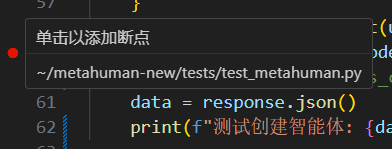
\includegraphics[width=0.8\textwidth]{images/breakpoints.png}
\caption{打断点的例子}
\end{figure}

这样就可以打出一个断点。在调试过程中,当程序执行到断点所在的行时,程序会暂停,我们可以查看当前的变量值和程序状态。我们可以通过单步执行(Step Over)来逐行执行代码,或者通过单步进入(Step Into)来进入函数内部进行调试。对于小型项目或者单文件项目,打断点是一个非常有效的调试手段。

\subsubsection{写测试代码}

写测试代码是指编写一些专门用于测试的代码,以便在运行时验证程序的正确性。测试代码可以帮助我们发现潜在的问题,并确保程序的功能正常。这也是用于较大型项目的调试手段,但是小型项目也可以使用。我们可以在这些测试代码中模拟各种可能出现的情况(包括常规值、边界值、异常值等),从而验证程序的正确性和健壮性。

测试代码通常分为单元测试和集成测试两种。单元测试是对程序的最小可测试单元进行验证,通常是函数或方法;而集成测试则是对多个单元进行组合验证,确保它们能够正常协同工作。

\begin{figure}[htbp]
\centering
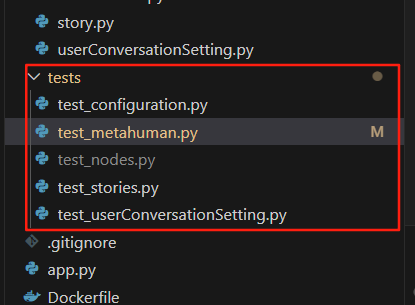
\includegraphics[width=0.8\textwidth]{images/tests.png}
\caption{我为本人实习的项目编写的集成测试}
\end{figure}

\subsubsection{小结}

debug 最重要的一件事是缩小错误出现的范围,为达成这一目的我们通常会跟踪代码的行为,直到发现代码的行为与预期不符。实际上最棘手的情况是,代码只在特定的数据上出现错误,尤其是当我们无法获取程序执行日志的时候。这种情况尤见于我们在POJ上做题的时候:POJ的测试数据是不可见的,只会告诉你结果是WA RTE还是TLE、MLE。

这时最应该做的是重新审视自己的预期(以及 OJ 题的题面),寻找是否遗漏了什么约束条件或关键信息。一份貌似运行正常的代码很有可能会在边界条件或复杂数据的情况下出问题,可以尝试手写一些处于边界条件之下的数据,或编写一个数据生成器来生成更复杂的数据。实在手足无措时,休息一下放空大脑也是很好的选择。实在走投无路之时,摇人求助也不是什么大不了的事情。debug 很可能会占用比编写代码更多的时间和精力,保持良好的心态才是 debug 的关键。

\subsection{维持代码风格}\label{sec:code-style}

代码风格(码风)是指代码的书写规范和格式化方式。良好的代码风格可以提高代码的可读性和可维护性,使得其他人(包括未来的自己)能够更容易地理解和修改代码。一般情况下,我们会遵循一些通用的代码风格规范,例如 Google C++ Style Guide 或 PEP 8(Python Enhancement Proposal 8)等。而在团队协作的时候,我们则尽可能保证码风和团队的码风一致。

一般情况下,有几个值得注意的点:
\begin{itemize}
  \item \textbf{缩进}:使用空格或制表符进行缩进,通常使用2个空格或4个空格或1个制表符。不要混用空格和制表符。
  \item \textbf{命名}:使用有意义的变量名和函数,不要使用单个字母或无意义的名称。同时,使用统一的命名风格,例如大驼峰(CamelCase)、小驼峰(camelCase)、下划线(snake\_case)等。
  \item \textbf{注释}:在代码中添加适当的注释,解释代码的逻辑和意图。注释应该简洁明了,不要过于冗长。同时,注释应该与代码保持同步,避免出现过时的注释。避免使用\texttt{\#if 0}和\texttt{\#endif}来注释代码,这种方式风格很老,现在已经不推荐使用了。
  \item \textbf{空行}:适当使用空行来分隔代码块。通常情况下,在类、函数之间使用一个空行,在逻辑相关的代码块之间使用两个空行;有时候在类、函数之间使用两个空行,而在逻辑相关的代码块之间使用\texttt{\#region}和\texttt{\#endregion}或者类似物来分隔代码块。(这取决于你使用的语言和编辑器)
  \item \textbf{括号}:使用一致的括号风格,例如 K\&R 风格(函数定义的左括号在同一行)或 Allman 风格(函数定义的左括号在新的一行)。注意不要在括号前面添加空格。
  \item \textbf{空格}:在运算符两边添加空格,例如\texttt{a + b}而不是\texttt{a+b}。在逗号、分号等符号后面添加空格,例如\texttt{a, b}而不是\texttt{a,b}。在函数调用时,函数名和左括号之间不添加空格,例如\texttt{func()}而不是\texttt{func ()}。
  \item \textbf{行长度}:尽量保持每行代码的长度在80-120个字符之间,避免过长的行导致代码难以阅读。可以使用换行符或者其他手段来分割长行。如果懒得数,也可以用半个屏幕为换行基准。
  \item \textbf{文件长度}:尽量保持每个文件的长度在1500行以内,避免过长的文件导致代码难以阅读。可以将相关的代码分成多个文件,或者使用模块化的方式来组织代码。
\end{itemize}

我们自己写代码的时候虽然不能强制要求自己遵循某种风格,但是在团队协作中,保持一致的代码风格是非常重要的。我们可以使用一些工具来自动格式化代码,VS Code的C++插件就提供了代码格式化功能,可以通过快捷键(通常是Shift + Alt + F)来自动格式化代码。而Python一般很少有代码格式化工具,我们要在自己书写时多加注意。

\end{document}